\documentclass{article}
% hiermit werden alle packages in eine separate .tex datei ausgeladen
% zum Einblenden von Grafiken
\usepackage{graphicx}
% ändert die automatisch generierten wörter (inhaltsverzeichnis etc.) zu deutsch. 
% default ist englisch, also einfach das includepackage löschen.
\usepackage[german]{babel}
% um Grafiken gezielt anzuzeigen mit /begin{figure}[H] /end{figure}
\usepackage{float}
%Quelltexthighlighting, integration dessen nicht als rastergrafik, sondern skalierbar
\usepackage{minted}

\usepackage[top=2cm, bottom=2cm, outer=0cm, inner=0cm]{geometry}
\usepackage[pages=some]{background}

\addbibresource{lit/lit.bib}

\begin{document}

% configuration für hintergründe der seiten
% command um ein hintergrundbild für alle seiten einzufügen, random kommentar im command um random leerzeichen raus zu kriegen
    % außerdem transparent mit hilfe eines weiteren packages
    %außerdem versch. hintergr. für gerade und ungerade seiten, wieder ein neues package
    \AddToShipoutPicture{%
        \ifthenelse
        {
            \isodd{
                \value{page}}
        }
        {%
            \transparent{0.2}
\includegraphics[width=\paperwidth, height=\paperheight]{graphics/backg02.jpg}
        }
        {%
            \transparent{0.2}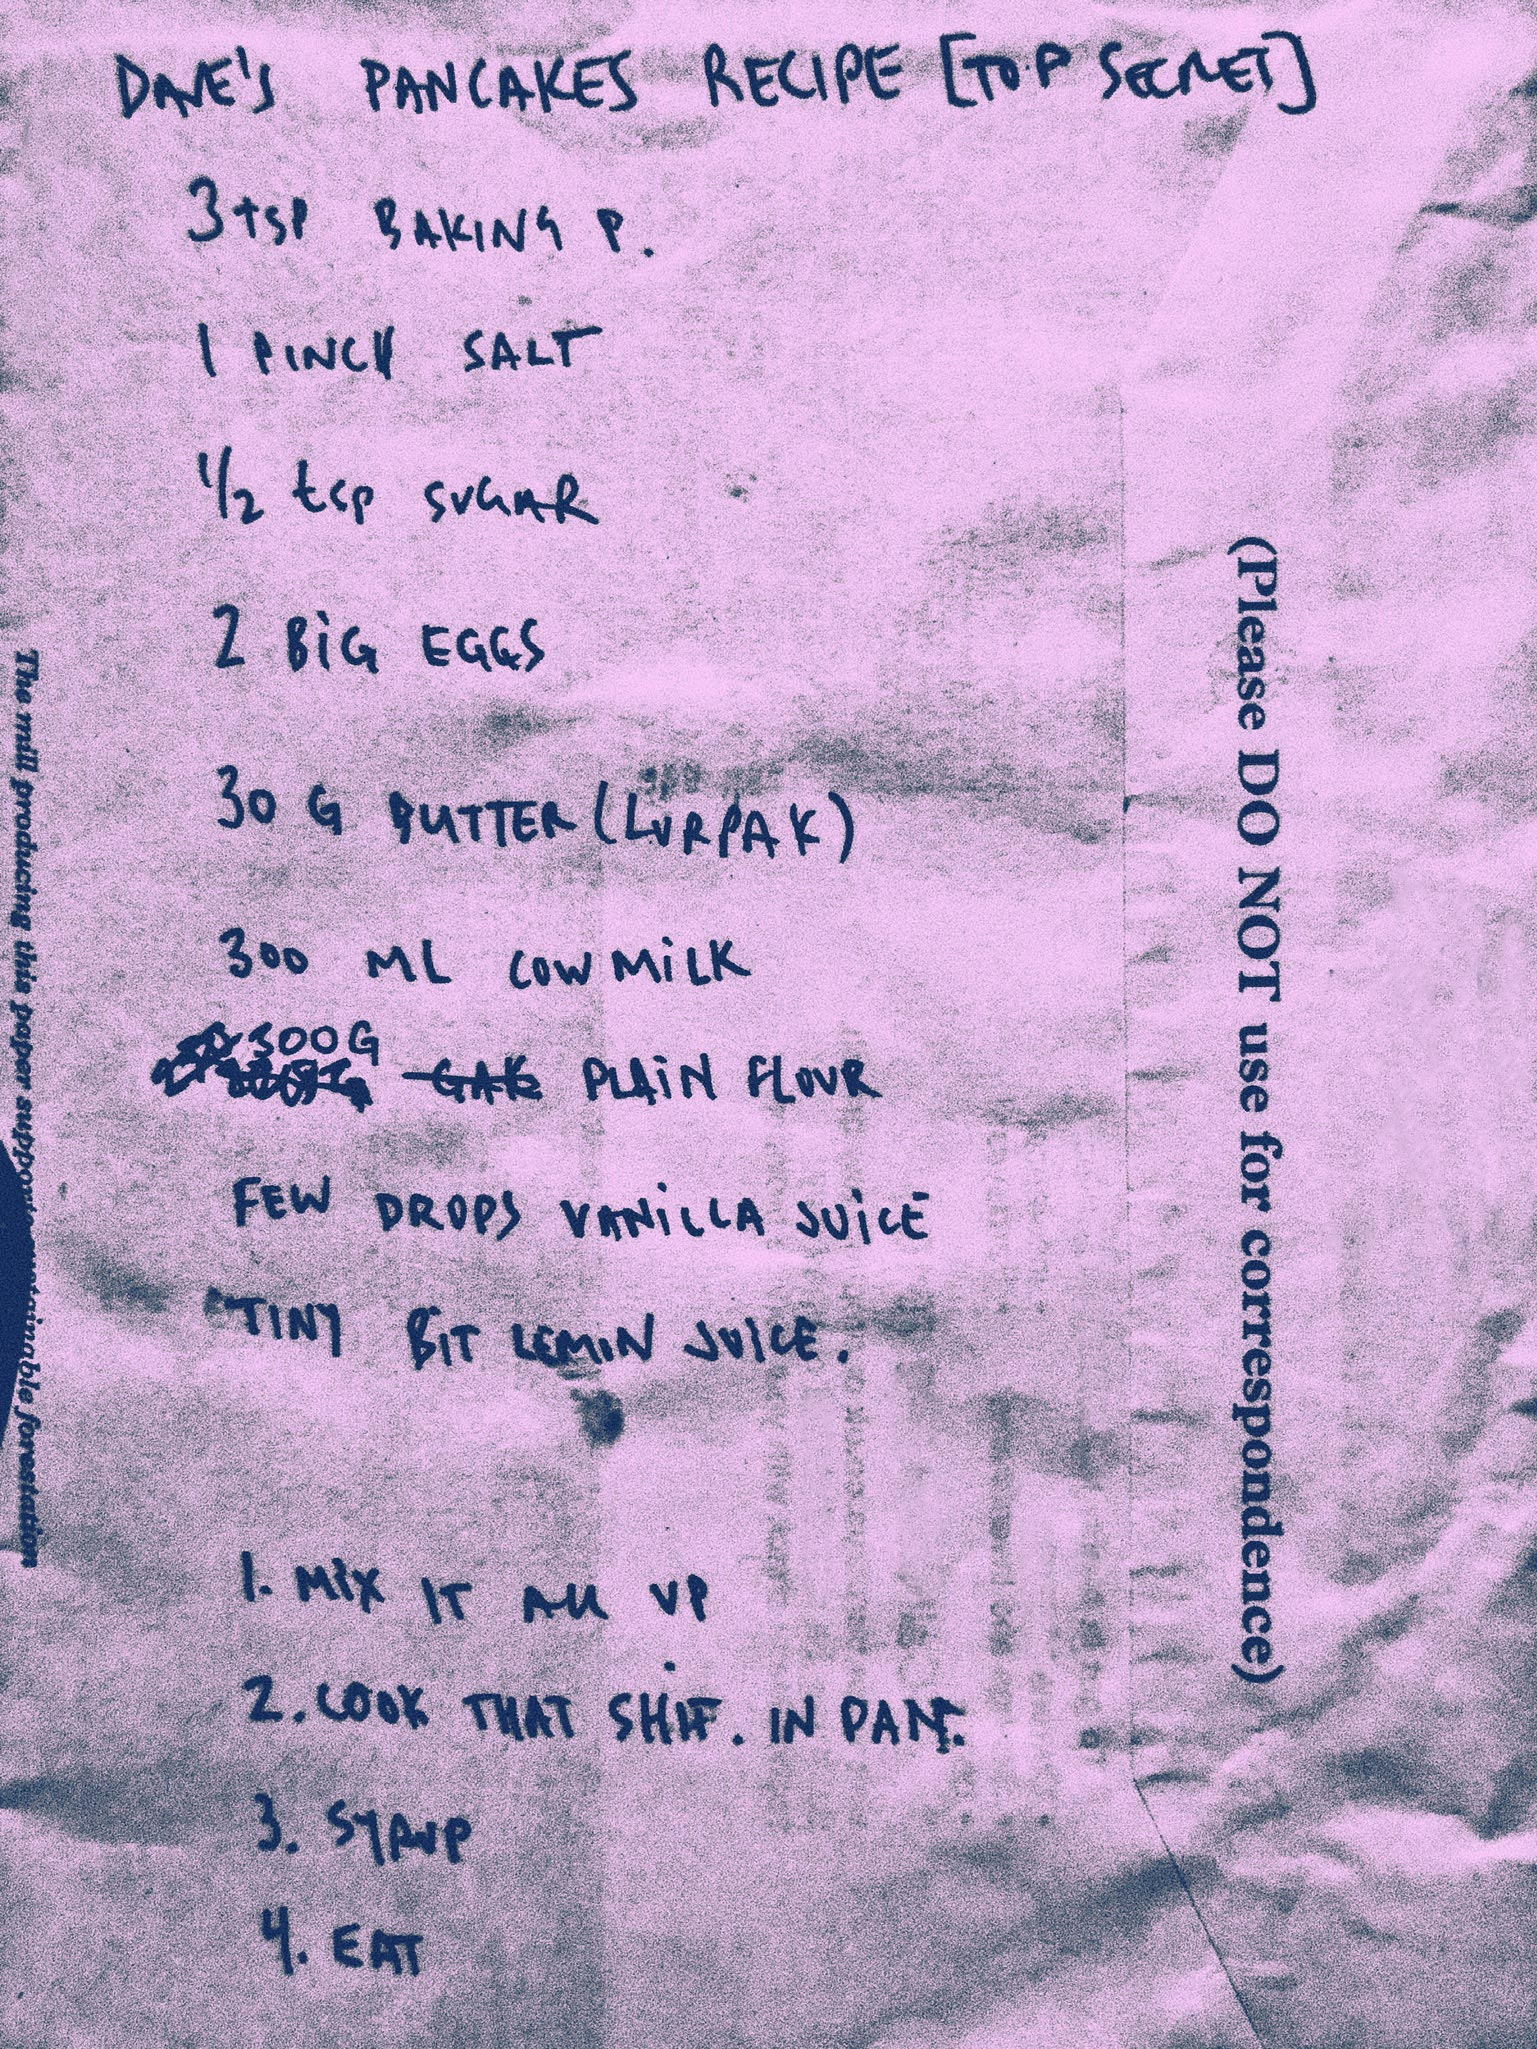
\includegraphics[width=\paperwidth, height=\paperheight]{graphics/DAVES_PANCAKES_RECIPE.jpg}
        }
    }
    
    % alle Seiten und Tabellen in Reihenfolge
    

    \begin{center}

        
\includegraphics[width=0.5\paperwidth]{graphics/logo black.jpg}
        \vspace{20mm}

        %mit huge können sachen sehr groß geschrieben werden, allerdings muss danach ein normalsize folgen
        % textsc, um ne nice überschrift mit kapitälchen zu schreiben
        \Huge{\textsc{Deckblatt}}
        \normalsize
    
        % und noch ein leerzeichen in das ding reinfeuern
        \vspace{20mm}
    
        % eine tabelle, um coole sachen geordnet darzustellen
        \begin{tabular}{r c l}
            Erstprüfer & Singer & Jürgen \\
            Zweitprüfer & Ackermann & Daniel \\
            Abgabedatum & 18. August & 2020 \\
        \end{tabular}
    
        % vfill für cooles einrichten einzelner elemente auf der seite.
        \vfill
        \begin{tabular}{r c l}
            Erstprüfer & Singer & Jürgen \\
            Zweitprüfer & Ackermann & Daniel \\
            Abgabedatum & 18. August & 2020 \\
        \end{tabular}
    
    
        
        % ohne das letzte vfill würde tabelle nach ganz unten eingerückt werden
        % \vfill 
    
    \end{center}
    % inhaltsverzeichnis
    \tableofcontents
    \newpage

    % abstand zwischen neuen absätzen erhöhen, am anfang des eigentlichen contents gelistet
    \parskip 8pt % andere einheiten px, em, ex und viele mehr

    \section*{Hinweise zur Abgabe} \label{chap:hinweise}
\addcontentsline{toc}{section}{Hinweise zur Abgabe}

In dieser mit Latex erstellten PDF sind folgende Inhalte enthalten: 

[Links in eckigen Klammern]

%eine schicke nicht numerierte Liste
\begin{itemize}
    \item Ein Deckblatt mit Titel, Datum, Prüfer, Matrikelnummer                               
    \item Ein Inhaltsverzeichnis      
    \item Wenigstens drei: 
        \begin{itemize}
            \item  Kapitel                                           
            \item  Unterkapitel                                                          
            \item  Unterunterkapitel
        \end{itemize}                                                                                                                   
    \item Wenigstens drei Paragraphen                                                           
    \item Wenigstens einem sub-Paragraphen                   [Siehe \nameref{chap:1}]                                   
    \item Ein Abbildungsverzeichnis                                                             
    \begin{itemize}                                                                             
        \item Mit wenigstens drei Bildern                                                       
        \begin{itemize}                                                                         
            \item Mit jeweils einem Untertitel                                                  
            \item Mit einem abweichenden kurzen Titel für das Abbildungsverzeichnis             
            \item Mit jeweils einer Referenzierung der Abbildung im Fließtext des Kapitels      
        \end{itemize}                                                                           
    \end{itemize}                                                                               
    \item Ein Listingsverzeichnis (nach Abbildungsverzeichnis)                                  
        \begin{itemize}                                                                         
            \item Mit wenigstens zwei Listings                                                  
                \begin{itemize}                                                                 
                    \item Mit Untertitel                                                        
                    \item Mit Abkürzung des UT für das Verzeichnis                              
                    \item Mit jeweils einer Referenz im Text darauf.                            
                \end{itemize}                                                                   
        \end{itemize}                                                                           
    \item Einen Anhang (nach Inhalt und Litverzeichnis)         [Siehe \nameref{chap:appendix}]                              
        \begin{itemize}                                                                         
            \item Mit wenigstens einer Abbildung                                                
            \item Mit wenigstens einem Listing                                                             
        \end{itemize}                                                                           
    \item Zwei wechselnde Hintergrundbilder (jede zweite Seite)                                            
    \item Ein Literaturverzeichnis vor Anhang und nach Inhalt
    
    \newpage
    
    \item Hervorgehobener Text      [Siehe \nameref{chap:2}]
        \begin{itemize}
            \item Kursiv
            \item Fett
            \item Unterstrichen
            \item In Anführungszeichen
        \end{itemize}
    \item Listen                
        \begin{itemize}
            \item Numeriert             [Siehe \nameref{chap:2}]
            \item Nicht numeriert       [Siehe \nameref{chap:hinweise}]
        \end{itemize}
    \item Zitate                   [Siehe \nameref{chap:1}]
        \begin{itemize}
            \item Indirekt
            \item Direkt 
            \item Zitat aus Internet mit Link der Webseite im Literaturverzeichnis
        \end{itemize}
    \item Eine \nameref{lab:eidesstattliche_erklaerung} mit Unterschrift als eingefügte PDF am Ende
\end{itemize}
    \section{Was ist ein Problem?} \label{chap:1}

% Paragraph
Diese Frage selbst stellt schon ein Problem dar. Konkreter sollten wir uns also Fragen: 
“Wie sieht ein Problem aus, welches ich mit der Ingenieurmethodik lösen kann?” 
\paragraph{Einfach ausgedrückt:} 
% eigentlich Subparagraph, Einrückung wird aber anscheinend durch \parindent oder ähnliches blockiert
Ein System mit ungewissen Attributen befindet sich in einem Zustand A und 
soll mit gegeben Ressourcen in einen besseren Zustand B versetzt werden. 
\subparagraph{Um diese recht einfache Definition} 

im Kern zu verstehen müssen jedoch einige Elemente in 
einen dringend notwendigen Kontext gestellt werden. So müssen wir, um eine Problematik mit 
der Ingenieurmethodik auf zu arbeiten folgende Begriffe definieren: Veränderung, Ressourcen, 
am Besten \& Ungewiss.

    \subsection{Veränderung}

    Veränderung ist der Übergang von einer Situation A in eine Situation B wobei sich Situation A von B 
    unterscheidet. In unserem Falle sind Situation A und B allerdings nicht fest definiert sondern müssen 
    erst erkannt werden. Herauszufinden wie Situation B aussieht und wie der Übergang herbei zu führen ist
    ist Aufgabe des Ingenieurs. Hierzu muss er allerdings Situation A möglichst genau definieren, eine
    Aufgabe die ihm selten vom Auftraggeber abgenommen wird, auch wenn er dies eigentlich tun sollte.
    So muss der Ingenieur erstmal das genaue Problem feststellen um dann für eben dieses Problem nicht 
    die Lösung sondern eine Lösung zu finden. Eben diese Lösung sollte dann die passendste aller
    möglichen Lösungen sein.


    \subsubsection{Am Besten}

    %hier handelt es sich um ein indirektes Zitat, weshalb in der Fußnote ein 'Vgl.' nicht fehlen darf
    Der Begriff “am Besten” ist im Falle des Ingenieurs nicht die ideale 
    Lösung des Problemes in einem ansonsten leeren Raum sondern ein möglichst optimaler Kompromiss 
    aus allen Faktoren und Kriterien. Da eben diese Kriterien von Person zu Person zumeist 
    unterschiedlich stark gewichtet werden ist es die Aufgabe des Ingenieurs die allgemeine 
    Gewichtung eben dieser Kriterien durch die Gesellschaft zu ermitteln. Da auch dies ein subjektiver 
    Prozess ist (bei dieser Evaluation  spielen die persönlichen Kriterien des Ingenieurs natürlich 
    auch eine Rolle) kann es keine ideale Lösung geben. Die “beste” Lösung die im Laufe dieses 
    Prozesses zu finden ist ist die, die möglichst viele Kriterien einfließen lässt und abhängig 
    der Gewichtung möglichst viele Teilnehmer zufriedenstellt. \footnote{Vgl. \cite[S. 35]{bock2001}}
       

    \subsubsection{Ungewissheit}

    %dies ist ein direktes zitat, weshalb das Vgl. in der Fußnote wegfällt
    \begin{quote}
        Ein großer Teil, nein, gar der Kern eines jeden Ingenieurs-Projektes ist es mit unvollständigen 
    Informationen auf ein schwammig definiertes Ziel mit unbekannt vielen Faktoren und Möglichkeiten 
    zu zu arbeiten. Wäre dies anders, also die Informationen vollständig, die Aufgabe klar definiert 
    und alle Faktoren bekannt wäre das Ganze nicht mehr als eine wissenschaftliche Formel zu lösen. 
    Alle Variablen werden Eingesetzt und am Ende steht das Ergebnis. Sollte sich im Laufe dessen 
    rausstellen dass sich Fehler eingeschlichen haben kann man diese korrigieren und die Variablen 
    nochmals einsetzen. Mögen sich eben diese Variablen auch ändern, die Formel und Prozedur bleiben 
    gleich. Eben diese Sicherheit ist bei einem Ingenieur-Problem jedoch nicht gegeben, da bis zum 
    Schluss kein vollständiges Bild der Ausgangs- und Endlage bekannt ist.
    Die Aufgabe des Ingenieurs ist es also diese Ungewissheit der Situation zu minimieren, in dem er 
    möglichst viele Faktoren und Kriterien in seine Überlegungen mit einfließen lässt und so einen 
    optimalen Kompromiss findet. \footnote{ \cite[S. 112]{koen2013}}
    \end{quote}
     


    \subsection{Der Kern des Ingenieursproblems}

    % hier wird von einer Webseite zitiert, deren Link im Literaturverzeichnis abgerufen werden kann
    Zusammengefasst sieht jedes Problem der Ingenieurmethodik wie folgt aus: Ein System mit 
    ungewissen Attributen befindet sich in einem Zustand A und soll mit gegebenen Ressourcen in 
    einen besseren Zustand B versetzt werden. \footnote{ \cite{method}}



    \section{Analyse} \label{chap:2}

%verschiedene Arten der Hervprhebung von Text
\textit{Die Aufgabe der Analysephase ist es, eingehendes Verständnis über alle Komponenten des Problemgebietes 
zu erlangen, sodass ein einzelnes, spezifisches und realistisches Ziel formuliert werden kann.}

\textbf{Das oberste Ziel der Analyse sollte immer sein, die vorerst viel umfassende und grobe Zielsetzung zu 
einer einzigen, spezifischen Aufgabe zu reduzieren. Die zuerst weite Problembeschreibung wird durch 
die Aufstellung leitender Thesen systematisch eingeschränkt, bis ein enges, aber hoch detailliertes 
Ziel im finalen Schritt der Analyse formuliert werden kann.}

    \subsection{Beschreibung des Problems}

    \underline{Projekte können in zwei Untergruppen eingeteilt werden.} Einerseits gibt es das Forschungsprojekt, 
    dessen Ziel die Gewinnung neuen Wissens ist. Daneben gibt es noch das Entwicklungsprojekt, bei dem 
    man bereits existierendes wissen nutzt, um ein neues Gerät zu entwickeln oder einen bestimmten 
    Effekt zu erzeugen. Häufig kann man ein Projekt allerdings nicht strikt zu einem der beiden 
    Gruppen zuordnen. Oftmals führt die Entwicklung eines neuen Geräts im Laufe seiner Entwicklungsphase 
    auch zu neuen Erkenntnissen. Manchmal ist es auch nötig ein neues Gerät zu entwickeln, damit neues 
    Wissen überhaupt zugänglich wird. Zweiteres trifft allerdings nur eher selten ein.
    Die Beschreibung eines Problems wird in der folgenden Grafik verdeutlicht.

    \begin{figure}[H]
        \centering
        % error 'overfull' = bild zu groß für platz, fixed indem man width auf das 0.x Fache anpasst (hier 0.5) 
        
\includegraphics[width=0.5\linewidth]{graphics/problem.jpg}
        \caption[Problemerkennung]{Der Moment des Erkennens eines Problems}

        
        %mit label werden grafiken in texts referenziert
        \label{fig:problemloesung}
    \end{figure}

    \newpage

    Sollte es schwer fallen, das Problem mit einer kurzen, präzisen Frage oder Aussage zu umschreiben, 
    enthält das Projekt möglicherweise mehr als ein Problem. Dies ist ein häufig auftretender Grund für 
    Verwirrung im Projektplan, denn unterschiedliche Probleme benötigen fast immer auch unterschiedliche 
    Lösungen. Die dadurch verworrenen und sich teilweise widersprechenden Projektziele können zu großen 
    Komplikationen führen und verheerende Auswirkungen auf den Erfolg des Projekts haben, sollten sie 
    sich auch durch die Restlichen Projektphasen ziehen.
    Daher sollte am Anfang der Analyse eine möglichst detaillierte Zusammenfassung des Problems 
    angefertigt werden. Darin beinhaltet sind auch ausreichende Hintergrundinformationen und eine 
    Motivation zur Behebung des Problems, um das Projekt im richtigen Kontext einordnen zu können.

    \subsection{Performance Kriterien festlegen}

    \enquote{Performance Kriterien sind Bedingungen, die jede vorgeschlagene Lösung zu einem Problem erfüllen muss.} 
    Ziel ist hier, den in der Abbildung \ref{fig:problemloesung} gezeigten Moment möglichst zu vermeiden. 
    Dabei sollte darauf geachtet werden, dass die Kriterien weder zu streng, noch zu offen sind. Das 
    Beispiel sei hier das Festlegen einer Deadline für einen Teil eines Projekts. Die vorgeschlagene 
    Lösung hier wäre drei Monate. Sind die Kriterien zu eng, würde das Projekt nach Ablauf der 
    festgelegten Zeit gestrichen werden, auch wenn die eigentliche Dauer gerade mal drei Monate und 
    ein Tag gewesen wären. Werden die Kriterien jedoch zu aussagelos gesetzt, könnte das Teilprojekt 
    potenziell nie ein Ende finden und das gesamte Projekt gerät in nicht aufholbaren Verzug. 
    Beide Ausgänge sind zu vermeiden. Die meisten Entwicklungsprojekte sind jedoch im Voraus schon von den 
    festen, strengen Bedingungen und Parametern der Anwendungsdomäne eingegrenzt. Das folgende Diagramm 
    \ref{fig:kriterien} liefert einen Überblick über die wichtigsten generell anerkannten Kriterien.


    \begin{figure}[H]
        \centering
        % error 'overfull' = bild zu groß für platz, fixed indem man width auf das 0.x Fache anpasst (hier 0.5) 
        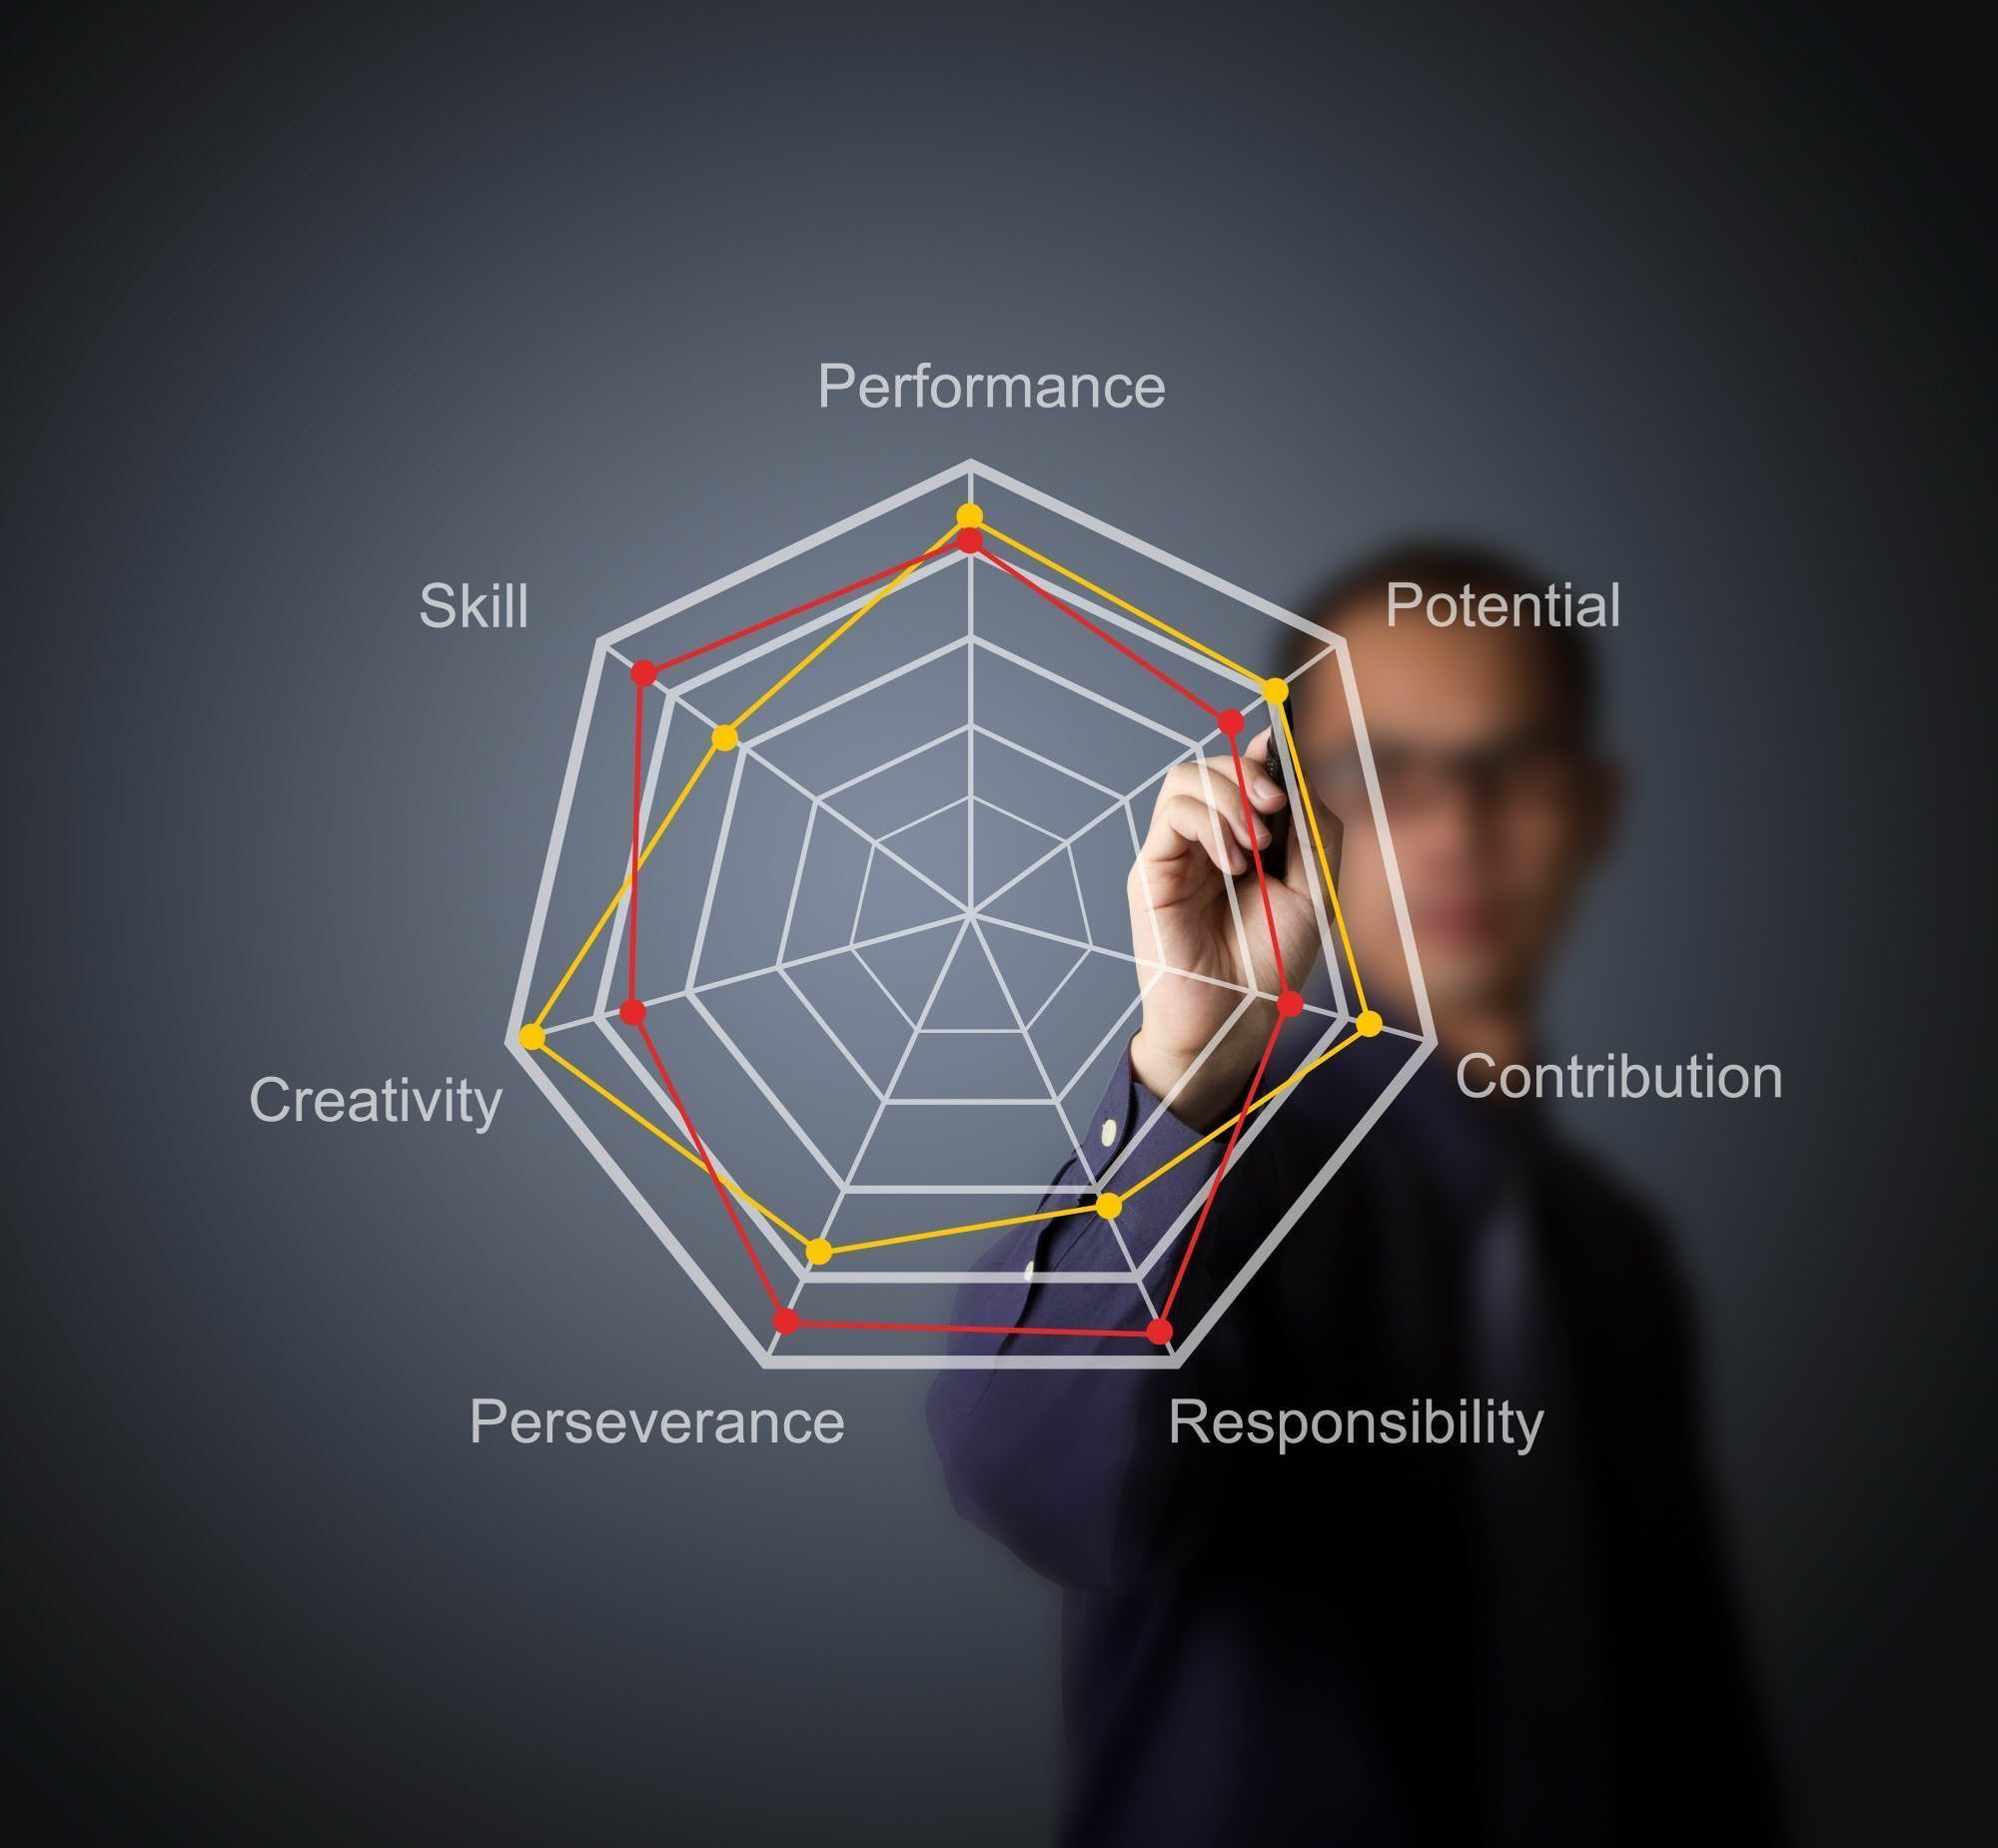
\includegraphics[width=0.4\linewidth]{graphics/kriterien.jpg}
        \caption[Performance Kriterien]{Die wichtigsten Performance Kriterien im Bereich des R\&D Sektors}

        
        %mit label werden grafiken in texts referenziert
        \label{fig:kriterien}
    \end{figure}

    \subsection{Themenverwandte Arbeiten untersuchen}

    Ist das Problem dann formal und präzise beschrieben und alle grundsätzlichen Performance 
    Kriterien festgelegt, so kann das Projektteam nun damit anfangen, möglichst viele Informationen 
    über vorhergehende Projekte in einem ähnlichen oder im gleichen Rahmen zu sammeln. Der wohl 
    bedeutendste Grund dafür ist es zu verhindern, “Das Rad neu zu erfinden.” Sollten 
    schon Lösungen für Teile, oder sogar das Projekt im Ganzen bestehen, ist es fast immer 
    einfacher und billiger die Lösung oder das Gerät zu kaufen, als der Versuch es zu replizieren. 
    Es gibt verschiedene Arten, um nach relevanten Quellen zu suchen. Einige davon sind hier 
    zusammengefasst:

        %eine schicke numerierte Liste
        \begin{enumerate}
            \item Professionelle Tagebücher
            \item Konferenzdokumentationen
            \item Bücher und Monographien
            \item Professionelle Studien 
            \item Zeitungsartikel
            \item Diskussionen mit Kollegen
            \item Reverse engineering
            \item Digitale Medien
                \begin{enumerate}
                    \item TV Berichte
                    \item Radiobeiträge
                    \item Ressourcen aus dem Internet
                        \begin{enumerate}
                            \item Webseiten
                            \item Datenbanken
                            \item Videos
                        \end{enumerate}
                \end{enumerate}
        \end{enumerate}
        

    Die Liste wird in Der Abbildung \ref{fig:medien} um weitere Punkte ergänzt.
    Unabhängig von der Quelle muss die validität immer gründlich überprüft werden. 
    Zweitquellen, wie z.B. Zeitungsartikel, müssen immer auf ihre ursprüngliche Quelle 
    zurückführbar sein, um die Echtheit der Information versichern zu können. Die Quellen, die 
    als Vorwissen in ein Projekt gebracht werden, müssen klar und strukturiert zitiert werden.

    \begin{figure}[H]
        \centering
        % error 'overfull' = bild zu groß für platz, fixed indem man width auf das 0.x Fache anpasst (hier 0.5) 
        
\includegraphics[width=0.5\linewidth]{graphics/media.jpg}
        \caption[Arten von Medien]{Ein Pfahl, der genau das gleiche wie der obige Text aussagt, nur cooler}

        
        %mit label werden grafiken in texts referenziert
        \label{fig:medien}
    \end{figure}

    \subsection{Ziel formulieren}

    Dies ist der letzte Schritt in der Analysephase. Nachdem das Problem klar definiert, die 
    Performance Kriterien festgelegt und verwandtes Material gründlich untersucht wurde, ist die 
    Aufgabendomäne nun angemessen fokussiert und eingegrenzt. Jetzt kann ein spezifisches und 
    klares Ziel für das Projekt bestimmt werden. Das Ziel ist ein Ausdruck von dem, was das Projekt 
    im Bestfall erreichen soll. Bevor zur nächsten Phase übergegangen wird, müssen noch zwei 
    Faktoren beachtet werden. 
    Als erstes, das Ziel ist die Basis, an der Erfolg oder Versagen des Projekts gemessen 
    werden. Auch die Leistung des Projektteams wird daran gemessen, wie gut es das Ziel erreicht hat. 
    Als zweites, auch wenn andere Komponenten des Projekts relativ unkompliziert angepasst 
    werden können, benötigt es für eine Änderung des Ziels explizite Erlaubnis der Management 
    Ebene, was zur Verschwendung großer Zeit- und Geldressourcen führen kann und deshalb vermieden 
    werden sollte. Umso wichtiger ist es, schon von Anfang an ein allgemein anerkanntes Ziel festzulegen.

    
    


    \section{Synthese} \label{chap:3}

Das Ergebnis der Synthesephase sollte die Anwendung der designten Lösung sein, um die gesetzten Ziele 
zu erreichen und die die Aufgabe begleitende Hypothese zu validieren.

Auch dieser Prozess kann in 4 kleinere Funktionen unterteilt werden aber anders als in der 
Analysephase, muss die Reihenfolge aller Schritte genau eingehalten werden. In dieser Phase werden 
alle vorher aufgestellten Thesen, Faktoren, Bedingungen, etc. mit Hilfe von Experimenten in die 
Praxis umgesetzt, um erste konkrete Ergebnisse zu erzielen.


    \subsection{Lösungsansätze implementieren}

    Es gibt zwei Arten, auf die eine Lösung implementiert werden kann, entwickeln und kaufen. 
    Ein Beispiel für eine selbst entwickelte Lösung kann im Listing \ref{lst:loesimpl} betrachtet werden.
    Sollte es den Anforderungen entsprechen, ist es fast immer effektiver die Lösung zu erwerben, 
    als sie selbst zu entwickeln. Dies trifft auch zu, sollte die erworbene Komponente nur zu einem 
    Teil zur Lösung beitragen. 
    Besteht ein Teil der Lösung aus einer Datenbank, sollte der Aufwand betrieben werden, um die Daten 
    vollständig, roh und unbearbeitet zu erhalten. Dies trifft vor allem zu, wenn die Daten von einer 
    anderen Forschungsgruppe oder Firma kommen. Häufig treten im Zusammenhang dessen auch politische 
    oder Eigentums Probleme auf. Von Drittparteien erhaltene Daten sollten generell immer mit einer 
    gewissen Skepsis behandelt werden.


    \begin{listing}[H]
        %caption wird benötigt, um das lisiting in das verzeichnis aufzunehmen, same mit abbildungen
        \caption[Loesungsimplementation Codebeispiel Java]{Beispiel einer Loesungsimplementation nach den festgelegten Vorschriften}
    % linenos -> numeriert zeilen, frame=lines -> grenzt code mit linien ab, fontsize -> schriftgröße, 
    % firstnumber -> zeile, in der snippet anfängt, muss al erster parameter stehen
    % unter den mathescape eingaben dann die gewählte sprache in {}
    % verfügbare sprachen via pygmentize dokumentation 
    \begin{minted}
        [
            firstnumber=5,
            frame=lines,
            framesep=2mm,
            baselinestretch=1.2,
            linenos
            ]
    {java} 
    
    package com.tutego.insel.ds.observer;
    
    import java.util.*;
    
    public class Party
    {
      public static void main( String[] args )
      {
        Observer achim    = new JokeListener( "Achim" );
        Observer michael  = new JokeListener( "Michael" );
        JokeTeller chris  = new JokeTeller();
    
        chris.addObserver( achim );
    
        chris.tellJoke();
        chris.tellJoke();
    
        chris.addObserver( michael );
    
        chris.tellJoke();
    
        chris.deleteObserver( achim );
    
        chris.tellJoke();
      }
    }
    
    \end{minted}
        \label{lst:loesimpl}
    \end{listing}


    \subsubsection{Experimente Designen}

    Der Sinn hinter diesem Schritt ist es, eine Reihe von Experimenten zu designen, dessen 
    Resultate benutzt werden, um zu messen wie gut eine Aufgabe erfüllt wurde. Ein Experiment 
    erfasst Daten um den Erfolg einer konzipierten Lösung unter kontrollierbaren Bedingungen im Labor 
    zu testen. Vor dem Beginn der Experimente sollten alle aufgestellten und gesammelten Faktoren, 
    Regeln, Bedingungen und Beobachtungen auf Vollständigkeit und Korrektheit überprüft werden, da 
    jede dieser Komponenten einen fundamentalen Einfluss auf die Planung und Durchführung der 
    Experimente haben kann.  Wurde diese Liste noch ein letztes mal verifiziert,  kann nun mit 
    der Planungsphase für die Experimente fortgefahren werden. 
    Zuerst sollte sichergestellt werden, dass das Labor, in dem das Experiment stattfinden wird, 
    frei von nicht-essentiellen Objekten ist. Der negative Einfluss von emotionalen Reaktionen der 
    Testsubjekte sowie der Prüfer kann oft nicht vollkommen verhindert werden. Deshalb sollte man 
    darauf achten, dass jedes Element im Labor unabdingbar für das Experiment ist. Einmal richtig 
    angeordnet, sollte danach großer Wert darauf gelegt werden, dass niemand außer den am Experiment 
    beteiligten Personen das Labor betritt. Außenstehende können ohne ihr Wissen kleinste Veränderungen 
    am Arbeitsraum durchführen, z.B. ein Gerät um wenige Millimeter verschieben, und damit die 
    Ergebnisse des Experiments vollkommen aussagelos machen. Das schlimmste daran ist, dass ein 
    solcher Fehler, wenn überhaupt, nur sehr schwer zurückverfolgt werden kann, wodurch das ganze 
    Projekt in Gefährdung stehen könnte. Deshalb sollte das Labor in Abwesenheit des Personals 
    immer verriegelt und klar und deutlich für Außenstehende gekennzeichnet sein, um die Chance 
    auf derartige Fehler zu minimieren. Das eigentliche Experiment besteht aus mehreren Elementen. 
    Angefangen wird bei dem Personal, dass das Experiment durchführen wird. Diese haben einen 
    genauen Überblick über alle bisher gesammelten Daten sowie die nötige Expertise um die 
    Experimente auch durchzuführen. Lebendige Teilnehmer eines Experiments werden Kohorte genannt, 
    ihr Gegenpol sind die Stichproben. Die Durchführung eines Versuchs mit einer schrittweisen 
    Veränderung der Faktoren, bis alle möglichen Faktorkombinationen abgedeckt sind, heißt Block 
    Design. Um die vorgesehene Funktion aller Faktoren bestätigen zu können, werden sogen. Control 
    Trials durchgeführt. Dabei wird die Performance von einem Set von Faktoren in Abwesenheit eines 
    anderen Sets von Faktoren gemessen, um die isolierten Effekte des Sets festhalten zu können. 

    Die aus Experimenten erhaltenen Daten sollten auf mehr als einem Medium gespeichert sein, um 
    den Verlust im Falle eines Ausfalls eines der Medien zu verhindern. Datenschutz sollte eine der 
    obersten Prioritäten sein. Am besten sollten fertig bearbeitete Daten irgendwo im Internetz gespeichert
    werden, damit sie für jeden zugänglich sind. Dies könnte mit Hilfe einer Webseite, wie im Listing
    \ref{lst:htmlex} passieren. Es empfiehlt sich, die Daten zu verschlüsseln und diesen Schlüssel 
    nur an die Personen weiterzugeben, die unbedingt Zugriff auf die Daten benötigen. Werden über 
    die schon bestehenden Speicherplätze der Daten hinaus weitere Kopien angefertigt, so muss dies 
    unbedingt Dokumentiert werden, um unkontrollierte Verbreitung der Daten zu verhindern. Sind alle 
    Daten einmal gespeichert, sollten diese umgehend mit Hilfe des Copyright weiter geschützt werden. 
    In der Regel ist es sinnvoll, zu viele Daten über das Experiment gespeichert zu haben als zu wenig.   

    \begin{listing}[H]
        %caption wird benötigt, um das lisiting in das verzeichnis aufzunehmen, same mit abbildungen
        \caption[Anzeigemoeglichkeit Experimente via HTML]{Die Grundlage einer HTML Seite, zum Teilen der designten Experimente}
    % linenos -> numeriert zeilen, frame=lines -> grenzt code mit linien ab, fontsize -> schriftgröße, 
    % firstnumber -> zeile, in der snippet anfängt, muss al erster parameter stehen
    % unter den mathescape eingaben dann die gewählte sprache in {}
    % verfügbare sprachen via pygmentize dokumentation 
    \begin{minted}
        [
            firstnumber=5,
            frame=lines,
            framesep=2mm,
            baselinestretch=1.2,
            linenos
            ]
    {html} 
    
        <!DOCTYPE html>
        <html>
            <body>

                <h1>My First Heading</h1>
                <p>My first paragraph.</p>

            </body>
        </html>
    
    \end{minted}
        \label{lst:htmlex}
    \end{listing}

    \subsubsection{Experimente durchführen}

    Jetzt gilt es nur noch, die bereits fertig geplanten Experimente durchzuführen. Dies 
    sollte genauestens nach Plan passieren, damit Fehler oder unerwartete Ergebnisse in den 
    Plänen gefunden und behoben werden können. Misslungene Experimente sollten als Hilfen 
    gesehen werden, um die Pläne zu überarbeiten und dem Erfolg einen Schritt näher zu kommen. 
    Um eine fehlerfreie 


    \subsubsection{Ergebnisse extrahieren}

    Oft können die direkten Ergebnisse eines Experiments nicht genutzt werden, um 
    Schlussfolgerungen zu ziehen. Zuerst müssen die Resultate reduziert werden, also 
    umgewandelt und kombiniert, damit die entstehenden Werte in Form der gewählten 
    Performance Metrik dargestellt werden können. Wurden bis jetzt alle Richtlinien beachtet, 
    sollten die Daten über einen simplen SQL Befehl, gezeigt im Beispiel \ref{lst:sqlex} ohne 
    weitere Probleme extrahiert werden können. Im Grunde können nur zwei Arten von 
    Werten direkt gemessen werden: Distanzen und Zählungen. Weil die reduzierten Daten oftmals 
    modifiziert oder korrigiert werden müssen, sollten immer die rohen und die reduzierten 
    Ergebnisse des Experiments dokumentiert werden.


    \begin{listing}[H]
        %caption wird benötigt, um das lisiting in das verzeichnis aufzunehmen, same mit abbildungen
        \caption[SQL Befehl, zur Extraktion der Ergebnisse]{SQL Befehl, um Ergebnisse aus dem Experiment zu extrahieren}
    % linenos -> numeriert zeilen, frame=lines -> grenzt code mit linien ab, fontsize -> schriftgröße, 
    % firstnumber -> zeile, in der snippet anfängt, muss al erster parameter stehen
    % unter den mathescape eingaben dann die gewählte sprache in {}
    % verfügbare sprachen via pygmentize dokumentation 
    \begin{minted}
        [
            firstnumber=5,
            frame=lines,
            framesep=2mm,
            baselinestretch=1.2,
            linenos
            ]
    {sql} 
    
    USE AdventureWorks2012;
    GO
    SELECT *
    FROM Production.Product
    ORDER BY Name ASC;
    -- Alternate way.
    USE AdventureWorks2012;
    GO
    SELECT p.*
    FROM Production.Product AS p
    ORDER BY Name ASC;
    GO
    
    \end{minted}
        \label{lst:sqlex}
    \end{listing}


    \newpage
    % abbildungsverzeichnis
    \listoffigures
    \newpage
    % listingverzeichnis
    \renewcommand{\listoflistingscaption}{Listingverzeichnis}
    \listoflistings
    \newpage
    % literaturverzeichnis
    \printbibliography

    \appendix 

\section*{Anhang}   \label{chap:appendix}
\addcontentsline{toc}{section}{Anhang}


% um numerierung im anhang trotzdem zu erhalten
\renewcommand{\thesubsection}{\Alph{subsection}}
% notation von abbildungen wird geänder: 1 > A.1 
\renewcommand{\thefigure}{\thesubsection.\arabic{figure}}
% an dieser stelle würde ich gern die notation von listings im anhang anpassen, bisher aber leider erfolglos

% berichtigen des counters für abbildungen
\setcounter{figure}{0}

\subsection{Nachbereitung}

Als allererstes, hier noch die letzte Referenz zum folgenden Listing im Anhang: \ref{lst:helloworld}  
Die hier benutzte Arbeit entstand im Rahmen des Moduls \textit{Wissenschaftliches Arbeiten} aus dem 
4. Semester. Da keine Bilder oder Grafiken vorgesehen waren, habe ich ein paar eher weniger relevante 
eingefügt. Trotzdem hoffe ich, dass der Leseflow der Arbeit einigermaßen angenehm ist. Alle für diese 
Abgabe relevanten Inhalte sind gleichmäßig über die Arbeit verteilt und können über die Seite 'Hinweise' 
angewählt werden. Überflüssige stellen der Arbeit wurden gelöscht, um den Inhalt bündig beisammen zu halten 
und nicht zu dünn zu verstreuen. Deshalb könnte der Text bei genauerem lesen allerdings auch teilweise 
nur wenig Sinn ergeben. 

    % großes H als kommando, damit content genau dort angezeight wird
    \begin{listing}[H]
        %caption wird benötigt, um das lisiting in das verzeichnis aufzunehmen, same mit abbildungen
        \caption[Java Hello World Beispiel]{Every java dev says 'Hello world!', but noone ever says 'How are you doing, world?'...}
    % linenos -> numeriert zeilen, frame=lines -> grenzt code mit linien ab, fontsize -> schriftgröße, 
    % firstnumber -> zeile, in der snippet anfängt, muss al erster parameter stehen
    % unter den mathescape eingaben dann die gewählte sprache in {}
    % verfügbare sprachen via pygmentize dokumentation 
    \begin{minted}
        [
            firstnumber=5,
            frame=lines,
            framesep=2mm,
            baselinestretch=1.2,
            linenos
            ]
    {java} 
    
        /*
        Java Hello World example.
        */
            
        public class HelloWorldExample{
            
          public static void main(String args[]){
            
            /*
            Use System.out.println() to print on console.
            */
            System.out.println("Hello World !");
            
          }
            
        }
            
        /*
        OUTPUT of the above given Java Hello World Example would be :
        Hello World !
        */
    
    \end{minted}
        \label{lst:helloworld}
    \end{listing}


\setcounter{figure}{0}
\subsection{Danksagungen}

Hier noch die letzte Anforderung an das Dokument in Form eines Bildes von unserem \nameref{fig:appendix_logo} im Anhang.

Lorem ipsum dolor sit amet, consetetur sadipscing elitr, sed diam nonumy eirmod tempor invidunt ut 
labore et dolore magna aliquyam erat, sed diam voluptua. At vero eos et accusam et justo duo dolores et 
ea rebum. Stet clita kasd gubergren, no sea takimata sanctus est Lorem ipsum dolor sit amet. Lorem ipsum 
dolor sit amet, consetetur sadipscing elitr, sed diam nonumy eirmod tempor invidunt ut labore et dolore 
magna aliquyam erat, sed diam voluptua. At vero eos et accusam et justo duo dolores et ea rebum. Stet 
clita kasd gubergren, no sea takimata sanctus est Lorem ipsum dolor sit amet. Lorem ipsum dolor sit
amet, consetetur sadipscing elitr, sed diam nonumy eirmod tempor invidunt ut labore et dolore magna
aliquyam erat, sed diam voluptua. At vero eos et accusam et justo duo dolores et ea rebum. Stet 
clita kasd gubergren, no sea takimata sanctus est Lorem ipsum dolor sit amet.   

 
    % großes H als kommando, damit content genau dort angezeight wird
    % aus einem unbekannten Grund führt die Verlinkung dieser Datei zu einer anderen Abbildung, obwohl 
    % die referenz die passende ist... könnte es am Renew Command für \thefigure liegen?
    % auch wenn \setcounter die nummern der abbildungen nicht zurück setzt, fängt das dokument trotzdem 
    % wieder neu an. es scheint, die tatsache, dass diese abbildung theoretisch wieder 'abbildung 1' ist, 
    % könnte der Grund für den Bug sein 
    \begin{figure}[H]
        \centering
        
\includegraphics[width=0.9\textwidth]{graphics/HSHARZ.png}
        \caption[Hochschullogo]{Das Logo unserer Hochschule}
        \label{fig:appendix_logo}
    \end{figure}

    % kommt immer ganz an ende
    % eidesstattliche als .tex seite 
   % % * entfernt numerierung an titel, exkludiert es aber auch aus inhaltsverzeichnis
\section*{Eidesstattliche Erklärung}
% hinzufügen zu inhaltsverzeichnis, allerdings ohne numerierung
% statt section könnte auch subsection benutzt werden, für andere ordnung im verzeichnis 
\addcontentsline{toc}{section}{Eidesstaatliche Erklärung}
%abstand 
\vspace{10mm}

Ich erkläre hiermit an Eides statt, dass ich die vorliegende Arbeit selbständig verfasst und dabei 
keine anderen als die angegebenen Hilfsmittel benutzt habe. Sämtliche Stellen der Arbeit, die im 
Wortlaut oder dem Sinn nach Publikationen oder Vorträgen anderer Autoren entnommen sind, habe ich 
als solche kenntlich gemacht. Die Arbeit wurde bisher weder gesamt noch in Teilen einer anderen 
Prüfungsbehörde vorgelegt und auch noch nicht veröffentlicht.

\vspace{10mm}

Wernigerode, den 18.08.1999

% einfügen mathematischer formel mit dollar zeichen, workaround für unterschrift
% tilden für länge des striches

% orientierung der formel nach rechts
\begin{flushright}
    $ \overline{ ~~~~~\mbox{Philipp Thüring} ~~~~~} $ 
\end{flushright}


   \ClearShipoutPicture
   % um nummer vor eintrag in verzeichnis zu löschen
   \setcounter{secnumdepth}{0}
   % eidesstattliche als pdf include
   %muss allerdings anders in verzeichnis geadded werden
   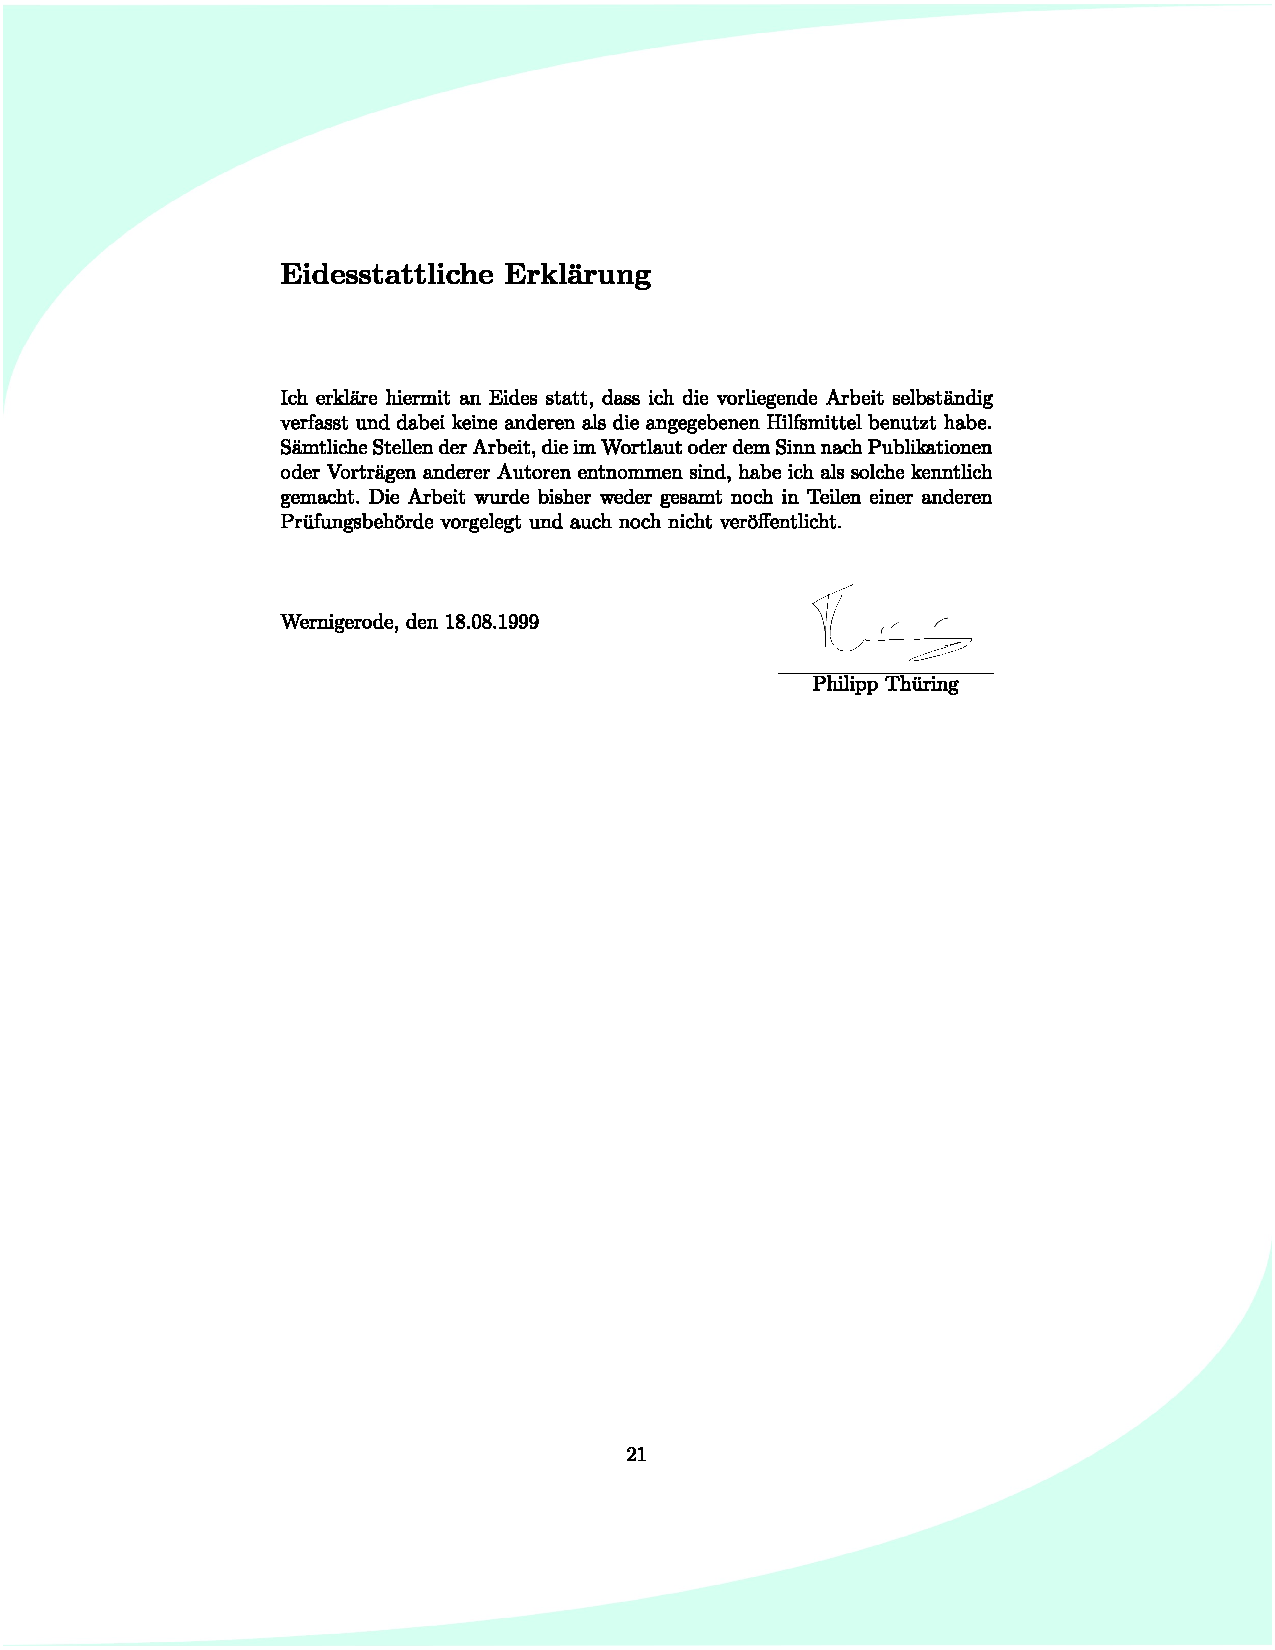
\includepdf[
        addtotoc={
            1, % seitennummer
            section, % section: sect. oder subsection
            1, % level: 1 (heißt section), 2 (heißt subsection)
            Eidesstattliche Erklärung, % heading: titel in toc
            lab:eidesstattliche_erklaerung % \ref
        }]{content/misc/erklaerung2.pdf}
   
\end{document}




